% !TeX program = pdflatex
% SIGMOD 2027 research submission layout, checked on 2026-09-30.
% Self-contained bilingual manuscript; English export: main-en.tex.
% Evidence: agent4db-adapter@743041f, experiments of 2026-09-29/30.
\documentclass[sigconf,review,anonymous]{acmart}
\newif\ifbilingual
\bilingualfalse
\ifbilingual
  \usepackage[UTF8,scheme=plain,fontset=fandol]{ctex}
\fi
\usepackage{amsmath}
\usepackage{booktabs}
\usepackage{tabularx}
\usepackage{tikz}
\usetikzlibrary{arrows.meta,positioning,fit}
\setcopyright{none}
\settopmatter{printacmref=false}
\citestyle{acmnumeric}
\newcommand{\system}{MAVRA}
\newcommand{\bi}[2]{#1\par\ifbilingual #2\par\fi}
\newcommand{\bt}[2]{#1\ifbilingual\space / #2\fi}
\newcommand{\bl}[2]{#1\ifbilingual\\#2\fi}
\newcommand{\code}[1]{\texttt{#1}}
\title{\system: Maintaining Shared Metric Definitions for Data Agents}
\ifbilingual
  \subtitle{面向数据智能体的共享指标定义维护}
\fi
\author{Anonymous Author(s)}
\begin{document}

\begin{abstract}
\bi{Sharing learned metric definitions can reduce repeated exploration by LLM data agents, but database updates can invalidate the data assumptions behind their implementations. Schema-only invalidation misses data-only failures, while definition-level on-demand revalidation repeats conditions shared by multiple definitions. We present \system, a middleware system that maintains shared metric definitions through executable validity conditions. It separates declared business semantics from filtered key uniqueness, join multiplicity, and time-role requirements, validates candidates extracted from judged-successful trajectories, and reuses condition verdicts across definitions at compatible dependency versions. Failed conditions trigger revocation and restricted, regression-tested repair; execution checks explicitly declared definition revisions. On synthetic retail data with one million sales rows, an eight-agent maintenance benchmark covers 19 definitions, four update events, and 80 configurations across forward and reverse policy orders. Condition-level maintenance uses 12.5--37.8\% of definition-level database time under staggered arrivals and 44.6--75.5\% under simultaneous arrivals, using the mean of the two per-order ratios. In a single-run DeepSeek experiment, maintained sharing answers 21/21 scored tasks correctly, versus 11/21 for middleware without shared definitions; maintenance database time is 22.36\,s versus 52.96\,s for definition-level revalidation. Both revalidation methods prevent observed stale-definition use. Schema-only maintenance executes six stale references and answers three post-update tasks incorrectly. These descriptive results support condition reuse, while concurrent repair availability and snapshot-bound execution remain open implementation issues.}
{共享已学习的指标定义能够减少大语言模型数据智能体的重复探索，但数据库更新可能破坏其实现所依赖的数据假设。只看表结构的失效策略会遗漏纯数据变化造成的错误，定义级按需重验证则会重复检查多个定义共享的条件。本文提出 \system，一种通过可执行有效性条件维护共享指标定义的中间层系统。它将显式业务语义与过滤后的键唯一性、连接多重性和时间角色要求分离，验证从判题成功轨迹中提取的候选，并在兼容的依赖版本上跨定义复用条件结论。条件失败触发撤销及经过回归测试的受限修复，执行端核对显式声明的定义修订。在含 100 万行销售记录的合成零售数据上，8 个智能体的维护实验覆盖 19 个定义、4 次更新，以及按正反策略顺序执行的 80 组配置。按两轮各自耗时比取平均，条件级维护在错峰到达时使用定义级数据库时间的 12.5--37.8\%，同时到达时为 44.6--75.5\%。单次 DeepSeek 实验中，维护后的共享口径答对 21/21 道计分题，无共享口径的中间层答对 11/21；维护数据库时间为 22.36 秒，定义级重验证为 52.96 秒。两种重验证方法均未观察到过期定义使用。只看结构的方法执行了 6 次过期引用，并答错 3 道更新后的题。这些描述性结果支持条件复用的价值；并发修复期间的可用性和绑定查询快照的执行仍是待完成的实现问题。}
\end{abstract}
\keywords{\bt{data agents, metric definitions, shared memory, validity conditions, database updates}{数据智能体，指标定义，共享记忆，有效性条件，数据库更新}}
\maketitle

\section{\bt{Introduction}{引言}}
\label{sec:introduction}
\bi{Data agents explore schemas, inspect values, test joins, and construct SQL to answer business questions. Repeating this process incurs database work and model reasoning, while independently generated queries can implement different meanings of the same metric. Agent-oriented data systems identify redundant exploration as an opportunity for sharing~\cite{liu2026agents}, and semantic memory makes earlier execution traces reusable~\cite{biswal2026agentsm}. Metric definitions capture which facts to aggregate, which business records to include, and how measurements relate across tables.}
{数据智能体通过探索表结构、检查取值、验证连接及构造 SQL 回答业务问题。重复探索会消耗数据库和模型推理资源，独立生成的查询还可能对同一指标采用不同口径。面向智能体的数据系统将重复探索视为共享的机会~\cite{liu2026agents}，语义记忆则使已有执行轨迹能够被复用~\cite{biswal2026agentsm}。指标定义记录应聚合哪些事实、纳入哪些业务记录，以及跨表的度量关系。}

\bi{Sharing turns a learned definition into long-lived state over a changing database. Its implementation relies on data properties: a filtered key identifies one business record, a join preserves the intended multiplicity, and a date relation uses the intended business role. These properties are not automatically enforced by the definition's SQL. Updates can break them without changing a table or column. The query still executes, but its aggregate can cease to implement the intended measurement.}
{共享会使学习得到的定义成为变化数据库上的长期状态。其实现依赖数据属性：过滤后的键对应一条业务记录，连接保持预期多重性，日期关联使用预期业务角色。这些属性不会由定义中的 SQL 自动保证。更新可能在不改变表或列的情况下破坏它们，查询仍能执行，但聚合结果可能偏离预期业务度量。}

\bi{Consider a returns table that initially contains one completed record per return. An ETL update appends an application-state record for an existing return. A definition that sums all rows now counts a business event twice. In our experiment, the unmodified single-period definition returns 6,588,699.86 instead of 3,294,349.93. Recovery requires identifying the broken grain condition, finding a filter consistent with completed returns, and validating a new revision against approved evidence.}
{例如，退货表最初对每笔退货只保留一条完成记录，ETL 随后为已有退货追加申请状态行。对所有行求和的定义便会重复计数。在本次实验中，未修改的单期定义返回 6,588,699.86，正确值为 3,294,349.93。恢复需要识别失效的粒度条件，找到符合已完成退货含义的过滤规则，并依据已认可的证据验证新修订。}

\bi{Schema-only invalidation misses this failure. Definition-level on-demand revalidation detects it but repeats work when several definitions share conditions. Lazy maintenance~\cite{zhou2007lazy} determines when to perform the work. A reusable condition determines its scope and how much evidence can be shared. A baseline that marks definitions pending and revalidates them remains usable after benign writes; avoiding unnecessary revocation is therefore not a claimed advantage over that baseline.}
{只看结构的失效策略无法发现这种错误。定义级按需重验证能够发现，但多个定义共享条件时会重复检查。懒维护~\cite{zhou2007lazy}决定何时维护，可复用条件决定维护范围及证据共享程度。将定义标为待验证并正确重查的基线在正常写入后仍可继续使用，因此本文不把避免不必要撤销作为相对该基线的优势。}

\bi{We present \system\ (\textbf{M}etric-\textbf{A}ware \textbf{V}alidation and \textbf{R}euse for \textbf{A}gents). Definitions with different formulas can share validity evidence. \system\ connects executable conditions to their data dependencies, reuses completed verdicts across definitions and agents, and shares compatible in-flight checks. Revision checks and restricted repair govern the use and replacement of shared knowledge. The paper makes three contributions:}
{本文提出 \system\（Metric-Aware Validation and Reuse for Agents，面向智能体的指标感知验证与复用）。不同公式的定义能够共享有效性证据。系统将可执行条件关联到数据依赖，跨定义和智能体复用已完成结论，并合并兼容的在途检查。修订检查与受限修复共同控制共享知识的使用和替换。本文有三项贡献：}
\begin{enumerate}
\item \bi{\textbf{An executable validity model.} Business definitions are coupled with typed conditions and grounded evidence, giving learned definitions a criterion for continued use.}
{\textbf{可执行有效性模型。}将业务定义与类型化条件、有依据的证据结合，为已学习定义的持续使用提供判断标准。}
\item \bi{\textbf{Condition-level maintenance.} Selective revalidation, completed-verdict reuse, and in-flight merging factor common validation and repair work out of individual definitions.}
{\textbf{条件级维护。}通过选择性重验证、已完成结论复用与在途合并，将共同验证和修复工作从各定义中提取出来。}
\item \bi{\textbf{Revision-aware use and empirical characterization.} Declared revisions are checked and failed definitions undergo regression-tested repair. Experiments separate correctness, database work, and availability; snapshot-bound execution is specified as a design extension.}
{\textbf{修订感知使用及实证分析。}核对声明修订，对失败定义执行经过回归测试的修复。实验分别分析正确性、数据库工作和可用性，并将绑定快照的执行明确作为设计扩展。}
\end{enumerate}

\section{\bt{Metric Definitions and Validity Conditions}{指标定义与有效性条件}}
\label{sec:model}
\subsection{\bt{Definitions and evidence}{定义与证据}}
\bi{A definition revision is represented conceptually as $m^r=(B,I,C,E,r)$, where $B$ is its business meaning, $I$ its structured implementation, $C$ a set of executable conditions, $E$ supporting evidence, and $r$ its revision identifier. The implementation records the fact table, aggregate expression, grain, time role, join references, persistent filters, and empty-input convention. Query parameters, such as the requested month, are separate from persistent filters.}
{定义修订可概念化为 $m^r=(B,I,C,E,r)$，其中 $B$ 为业务含义，$I$ 为结构化实现，$C$ 为可执行条件集，$E$ 为支撑证据，$r$ 为修订号。实现记录事实表、聚合表达式、粒度、时间角色、连接引用、持久过滤和空输入约定。查询参数（如月份）与持久过滤分开。}

\bi{Evidence includes the source task, explicit business-definition basis, tool results, a task-success judgment, and database-version information. Answer production and successful SQL execution do not imply verified completion. The experiments use hand-written reference queries independent of the agent's answer but sharing the workload generator; they are not an externally certified business standard. Applications would need approved business tests or confirmed examples.}
{证据包括来源任务、显式业务定义依据、工具结果、任务成功判定及数据库版本信息。产出答案或成功执行 SQL 不等于任务通过验证。实验以手写参考查询判题，独立于智能体答案但与负载生成器同源，并非外部认证的业务标准；实际应用需要已认可的业务测试或确认示例。}

\subsection{\bt{Conditions and their scope}{条件及其范围}}
\bi{Let $D_s$ denote database snapshot $s$. A condition $c$ is a predicate over the tables in $\operatorname{dep}(c)$. The model distinguishes the following requirements.}
{记 $D_s$ 为数据库快照 $s$。条件 $c$ 是其依赖表集合 $\operatorname{dep}(c)$ 上的谓词，模型区分以下要求。}
\begin{description}
\item[\bt{Filtered key uniqueness}{过滤后键唯一性}]
\bi{The selected key identifies at most one relevant row under the declared filter and null policy.}
{在声明的过滤与空值规则下，所选键最多对应一条相关记录。}
\item[\bt{Join multiplicity}{连接多重性}]
\bi{The join direction, keys, and required filters preserve the permitted number of matches per fact.}
{连接方向、键和必需过滤应保持每条事实记录允许的匹配数。}
\item[\bt{Coverage and time role}{覆盖与时间角色}]
\bi{Required business keys remain represented and dates use the intended relation. Coverage requires an explicit population and tolerance; full independent coverage maintenance extends beyond the evaluated grain and join checks.}
{要求覆盖的业务键总体保持可表示，日期通过预期关系关联。覆盖需要显式总体和容差；完整的独立覆盖维护超出本次评估的粒度与连接检查。}
\end{description}

\subsection{\bt{Pending validation and revocation}{待验证与撤销}}
\bi{A dependency change makes relevant validation pending; it does not itself prove a definition invalid. Passing revalidation refreshes evidence. A failed required condition revokes the revision, and repair creates a candidate replacement. For a snapshot-bound realization, the intended admission contract is}
{依赖变化使相关验证进入待验证状态，本身不证明定义失效。重验证通过后刷新证据，必需条件失败则撤销修订，修复产生候选替代。对绑定快照的实现，预期准入契约为}
\begin{equation}
\begin{split}
\operatorname{Admit}(q,m^r,s)\Longrightarrow {}& \operatorname{Available}(m^r,s)\\
&{}\land\bigwedge_{c\in C(m^r)}c(D_s).
\end{split}
\end{equation}
\bi{The contract governs explicitly declared revision use, not arbitrary SQL correctness, and requires validation and execution on the same snapshot. Section~\ref{sec:execution} distinguishes that design from the prototype. Canonical compilation and answer evaluation separately address adherence to business semantics.}
{该契约约束显式声明的修订使用，不能等同于任意 SQL 正确性，并要求验证与执行使用同一快照。第~\ref{sec:execution} 节区分此设计与原型。规范查询编译及答案评估另行判断是否遵守业务语义。}

\section{\bt{System Overview}{系统概览}}
\label{sec:overview}
\bi{Figure~\ref{fig:architecture} separates learning admission, shared maintenance, and execution. The Rust adapter exposes tool-style HTTP endpoints for exploration, join validation, metric lookup, and SQL execution. Its in-memory store contains versioned definitions and supporting knowledge. Table fingerprints, DML statistics, and ETL batches drive dependency-version detection. The optional check-order optimizer is outside this comparison.}
{图~\ref{fig:architecture}区分学习准入、共享维护和执行。Rust 中间层通过工具风格的 HTTP 接口提供探索、连接验证、指标查找及 SQL 执行，内存知识库保存版本化定义和支撑知识。表指纹、DML 统计和 ETL 批次驱动依赖版本检测。可选的检查顺序优化器不属于本次比较。}

\begin{figure*}[t]
\centering
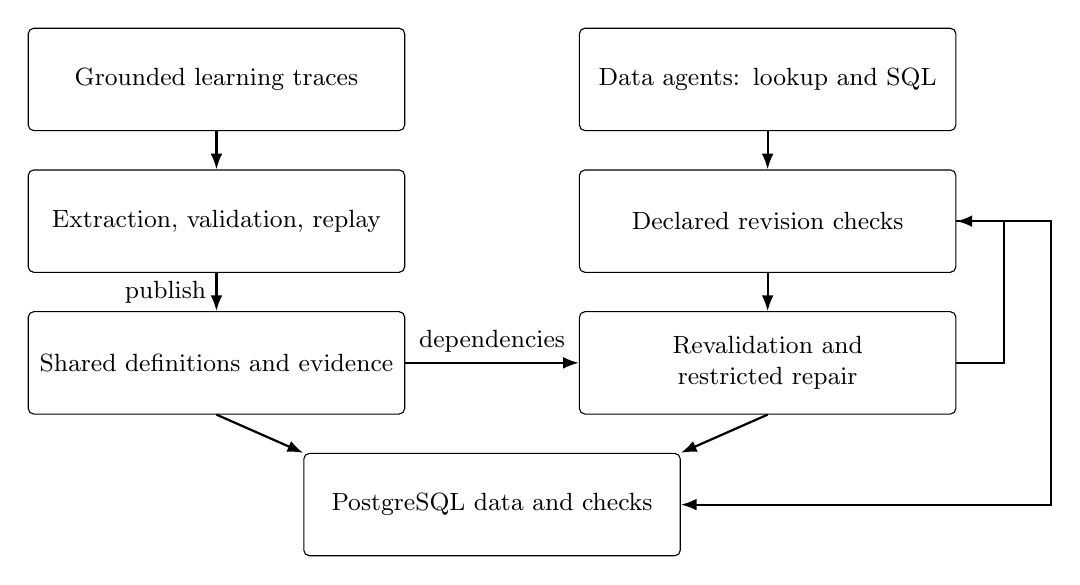
\begin{tikzpicture}[
box/.style={draw,rounded corners=2pt,align=center,minimum height=13mm,text width=45mm,font=\small,inner sep=4pt},
flow/.style={-{Latex[length=2mm]},thick},every node/.style={font=\small}]
\node[box] (learning) at (0,0) {\bl{Grounded learning traces}{有业务依据的学习轨迹}};
\node[box] (agents) at (7,0) {\bl{Data agents: lookup and SQL}{数据智能体：查找与 SQL}};
\node[box] (admission) at (0,-1.8) {\bl{Extraction, validation, replay}{提炼、验证与重放}};
\node[box] (execution) at (7,-1.8) {\bl{Declared revision checks}{声明修订核对}};
\node[box] (store) at (0,-3.6) {\bl{Shared definitions and evidence}{共享定义与证据}};
\node[box] (maintenance) at (7,-3.6) {\bl{Revalidation and restricted repair}{重验证与受限修复}};
\node[box] (database) at (3.5,-5.4) {\bl{PostgreSQL data and checks}{PostgreSQL 数据与检查}};
\draw[flow] (learning) -- (admission);
\draw[flow] (agents) -- (execution);
\draw[flow] (admission) -- node[left,align=center]{\bl{publish}{发布}} (store);
\draw[flow] (store.east) -- node[above,align=center]{\bl{dependencies}{依赖}} (maintenance.west);
\draw[flow] (execution) -- (maintenance);
\draw[flow] (maintenance.south) -- (database.north east);
\draw[flow] (store.south) -- (database.north west);
\draw[flow] (maintenance.east) -- ++(0.6,0) |- (execution.east);
\draw[flow] (execution.east) -- ++(1.2,0) |- (database.east);
\end{tikzpicture}
\caption{\bt{\system\ architecture. Admission publishes validated definitions; maintenance shares evidence; execution checks declared revisions.}{\system\ 架构：准入发布已验证定义，维护共享证据，执行核对声明修订。}}
\label{fig:architecture}
\Description{Learning feeds admission and a shared store. Agents feed revision checks and maintenance. Both paths access PostgreSQL.}
\end{figure*}

\bi{Different formulas can share the same condition. Revenue and return rate may require the same sales-grain check. A completed verdict serves both at compatible dependency versions; concurrent requests share an in-flight computation. Completed-verdict reuse and in-flight merging are controlled separately in the evaluation.}
{不同公式能够共享条件，例如营业额与退货率依赖同一销售粒度检查。兼容依赖版本上的已完成结论可供两者使用，并发请求共享在途计算。评估对已完成结论复用与在途合并分别控制。}

\section{\bt{Admission and Condition Maintenance}{准入与条件维护}}
\label{sec:maintenance}
\subsection{\bt{Admission from successful trajectories}{从成功轨迹准入}}
\bi{Candidates are extracted only from tasks with explicit business evidence and a successful judgment. Gates G1--G7 check business evidence, provenance and calculation chains, static well-formedness, grain, SQL review, example replay, and canonical-query replay. Learning questions supply admission evidence; held-out questions measure transfer. Current replay uses version checks and reference queries rather than a transactionally bound admission snapshot.}
{只从具备显式业务依据且判题成功的任务中提取候选。G1--G7 检查业务依据、结果来源及计算链、静态合法性、粒度、SQL 审查、示例重放和规范查询重放。学习题提供准入证据，留出题测量迁移。当前重放使用版本核对和参考查询，尚未绑定事务性准入快照。}

\subsection{\bt{Condition identities and dependencies}{条件身份与依赖}}
\bi{A condition identity includes its check type, table, keys, join direction, filters, and null policy. Sharing requires equality under supported normalization or a justified implication; textual similarity is insufficient. A reusable verdict is conceptually indexed by}
{条件身份包括检查类型、表、键、连接方向、过滤和空值规则。共享要求在支持的规范化下相等或满足有依据的蕴含，仅文本相似不足以共享。可复用结论概念上以如下键索引：}
\[
\bigl(\operatorname{id}(c),V(\operatorname{dep}(c))\bigr).
\]
\bi{Here $V$ is the detected dependency version. Referenced join revisions also propagate changes to definitions. These versions support prototype maintenance but do not establish equivalence between arbitrary database snapshots.}
{其中 $V$ 是检测到的依赖版本。引用的连接修订变化也会传播到定义。这些版本支撑原型维护，但不能证明任意数据库快照等价。}

\subsection{\bt{Selective revalidation and reuse}{选择性重验证与复用}}
\bi{On use, the adapter rechecks conditions whose dependencies changed, retains evidence over unchanged tables, and reuses compatible completed verdicts. Otherwise, compatible concurrent requests share a check. The definition-level baseline rechecks the entire condition set and forces join guards to rerun, using identical conditions, repair, regression, and in-flight merging.}
{使用时，中间层重查依赖变化的条件，保留未变化表上的证据，并复用兼容的已完成结论；否则，兼容的并发请求共享检查。定义级基线重查全部条件并强制重跑连接守卫，同时使用相同条件、修复、回归和在途合并。}

\bi{Under identical filters and null semantics, uniqueness on a subset of key columns implies uniqueness on a superset. This restricted implication does not cross incompatible populations. Repair searches over the same table and business key can also share a candidate filter, subject to revalidation and regression.}
{过滤及空值语义相同时，键列子集上的唯一性蕴含其超集上的唯一性。该受限蕴含不跨越不兼容总体。同表、同业务键的修复搜索也可共享候选过滤，但仍需重验证与回归。}

\subsection{\bt{Revocation and restricted repair}{撤销与受限修复}}
\bi{A failed condition revokes the revision and records a reason. Repairs are restricted to supported filters and revalidated join paths. Restoring uniqueness alone does not establish business meaning. Before publication, a candidate repeats static, grain, and SQL checks and passes G8 regression against learning evidence on current data. Failed repair leaves it unavailable.}
{条件失败撤销修订并记录原因，修复限定在支持的过滤与重新验证的连接路径内。恢复唯一性本身不证明业务含义正确。候选发布前需重复静态、粒度及 SQL 检查，在当前数据上通过基于学习证据的 G8 回归；失败则保持不可用。}

\bi{Repair can finish in the triggering request. Some concurrent arrivals instead observe a revoked state while repair is running. Section~\ref{sec:availability} measures this availability gap; the prototype does not yet make every such arrival wait for the repair outcome.}
{修复可在触发请求中完成，但部分并发请求在修复进行时看到撤销状态。第~\ref{sec:availability} 节测量这一可用性缺口，原型尚未让所有此类请求等待修复结果。}

\section{\bt{Revision-Aware Execution}{修订感知执行}}
\label{sec:execution}
\bi{Agents declare metric keys and revisions used by a query. Checks reject absent, revoked, inaccessible, or superseded references, and SQL review checks supported structural requirements. A retrieved definition is checked again when explicitly declared SQL relies on it. Undeclared use and arbitrary adherence to the business formula remain outside the revision-check guarantee.}
{智能体声明查询所用指标键及修订号。检查拒绝不存在、已撤销、不可访问或已被替代的引用，SQL 审查核对支持的结构要求。检索出的定义在显式声明的 SQL 使用时再次核对。未声明使用及任意 SQL 是否遵守业务公式超出修订检查的保证范围。}

\bi{A stronger snapshot-bound protocol acquires a query snapshot, resolves declared revisions and compatible evidence, validates remaining conditions against that snapshot, and executes on the same snapshot. Replacements require renewed resolution and declaration. A stable transaction or exported snapshot can realize this protocol. Cross-snapshot reuse additionally needs evidence of unchanged dependency data. TxCache provides precedent for consistent cached reuse~\cite{ports2010txcache}.}
{更强的绑定快照协议获取查询快照，解析声明修订及兼容证据，在该快照上验证剩余条件，并在同一快照上执行。使用替代修订需重新解析和声明。稳定事务或导出快照可实现该协议，跨快照复用还需依赖数据未变化的证据。TxCache 提供了一致性缓存复用的技术先例~\cite{ports2010txcache}。}

\bi{The evaluated prototype checks before execution but does not bind validation and business SQL to one repeatable-read transaction. Experiments use controlled update phases rather than adversarial concurrent writers. Absence of observed stale use is therefore an empirical result for those phases, not a proved snapshot-consistency guarantee.}
{被测原型在执行前检查，但未将验证和业务 SQL 绑定到同一个可重复读事务。实验采用受控更新阶段，没有对抗性的并发写入。因此，未观察到过期使用是这些阶段下的实证结果，不是已证明的快照一致性保证。}

\section{\bt{Evaluation}{实验评估}}
\label{sec:evaluation}
\subsection{\bt{Environment and questions}{环境与研究问题}}
\bi{We ask whether maintenance detects data-only failures, how much condition reuse saves beyond definition-level revalidation, how arrivals affect the gain, and whether learned sharing transfers to another agent. The machine has 48 Hygon cores and 98\,GiB RAM. PostgreSQL 18.6 runs with WAL and fsync disabled in disposable isolated databases. Synthetic retail data uses TPC-DS-style column names, not an official TPC-DS benchmark: one million store-sales rows, about 396,000 returns, and 500,000 catalog-sales rows.}
{实验研究维护能否检测纯数据变化失效、条件复用相对定义级节省多少、到达方式如何影响收益，以及共享学习结果能否迁移到另一智能体。实验机有 48 核 Hygon 和 98\,GiB 内存。PostgreSQL 18.6 在可丢弃的隔离库中运行，关闭 WAL 与 fsync。合成零售数据采用 TPC-DS 风格列名，并非官方 TPC-DS 基准，含 100 万行门店销售、约 39.6 万行退货和 50 万行目录销售。}

\bi{Benign events append sales, returns, and catalog sales. The breaking event v2 appends 170,816 application-state rows for returns dated from 2001-10-01 without changing the schema. It breaks ticket-and-item uniqueness; repair adds a completed-status filter. These are four update events, three benign and one data-only breaking, not four independently varied failure classes.}
{正常事件分别追加门店销售、退货和目录销售。破坏性事件 v2 为 2001-10-01 起的退货追加 170,816 条申请状态行，表结构不变。小票与商品键上的唯一性被破坏，修复添加完成状态过滤。这是 4 次更新事件，3 次正常、1 次纯数据破坏，不是 4 类独立变化的故障。}

\begin{table}[t]
\caption{\bt{Maintenance methods. Revalidation methods share conditions, repair, regression, and in-flight merging.}{维护方法：重验证方法具有相同条件、修复、回归与在途合并。}}
\label{tab:baselines}
\begin{tabularx}{\linewidth}{@{}lX@{}}
\toprule
\bt{Method}{方法} & \bt{After a dependency update}{依赖更新后}\\
\midrule
\bt{Schema}{结构} & \bt{Check structure only.}{仅检查结构。}\\
\bt{Revoke}{撤销} & \bt{Revoke and relearn.}{撤销并重学。}\\
\bt{Definition}{定义级} & \bt{Recheck all conditions on use.}{使用时重查全部条件。}\\
\bt{Scope}{范围} & \bt{Recheck affected conditions, no verdict reuse.}{重查受影响条件，不复用结论。}\\
\bt{Condition}{条件级} & \bt{Scope plus verdict and repair reuse.}{范围加结论及修复复用。}\\
\bottomrule
\end{tabularx}
\end{table}

\subsection{\bt{Controlled maintenance benchmark}{受控维护实验}}
\bi{Definitions are admitted directly through validation gates without LLM extraction. Four families contain six sales definitions, five returns definitions, three return-ratio definitions, and five catalog definitions. Taking up to $k\in\{1,2,4,6\}$ per family yields 4, 8, 15, and 19 definitions. After each update, eight scripted agents each use every definition in shuffled order. Arrivals are staggered or simultaneous. Five policies, four sharing levels, and two arrival modes yield 40 cells; forward and reversed policy orders yield 80 cells. These are two order-controlled passes, not independent repeated trials for confidence intervals.}
{定义直接通过验证门槛准入，不调用模型提炼。四个族包含 6 个销售、5 个退货、3 个退货比率及 5 个目录指标。每族最多取 $k\in\{1,2,4,6\}$ 条，对应 4、8、15 和 19 个定义。更新后，8 个脚本智能体各按打乱的顺序使用所有定义，采用错峰或同时到达。5 种策略、4 个共享度和 2 种到达方式构成 40 组，正反策略顺序共 80 组。这是两轮顺序控制实验，不是用于置信区间的独立重复试验。}

\bi{Database time sums actual operations during post-update uses, including maintenance and version reads, but excludes admission. Waiting sums uses that perform or join maintenance; under simultaneous arrivals it is aggregate agent waiting, not benchmark elapsed time. Stale use means a revision returned as valid whose canonical SQL fails a current-data probe. False revocation and unavailable use are separate counts.}
{数据库时间累计更新后使用期间的实际操作，包含维护及版本读取，不含准入。等待累计执行或合并维护的使用耗时，同时到达时是智能体等待之和，不是实验墙钟时间。过期使用指返回为有效的修订，其规范 SQL 未通过当前数据探测。误撤销和不可用单独计数。}

\begin{table*}[t]
\caption{\bt{Maintenance DB-time ratios relative to definition-level revalidation. Means are arithmetic means of the two per-order ratios. Scope means omit completed-verdict reuse.}{相对定义级的维护数据库耗时比：平均值为正反两轮各自比值的算术平均，范围组不复用已完成结论。}}
\label{tab:sharing}
\begin{tabularx}{\textwidth}{@{}Xrrrrr@{}}
\toprule
\bt{Arrival}{到达} & $k$ (\bt{definitions}{定义数}) & \bt{Forward}{正序} & \bt{Reverse}{反序} & \bt{Mean}{平均} & \bt{Scope mean}{范围组平均}\\
\midrule
\bt{Staggered}{错峰} & 1 (4) & 39.1\% & 36.4\% & 37.8\% & 89.3\%\\
 & 2 (8) & 23.3\% & 19.5\% & 21.4\% & 76.1\%\\
 & 4 (15) & 15.5\% & 16.2\% & 15.8\% & 82.7\%\\
 & 6 (19) & 12.5\% & 12.5\% & 12.5\% & 80.7\%\\
\midrule
\bt{Simultaneous}{同时} & 1 (4) & 63.9\% & 73.0\% & 68.4\% & 84.0\%\\
 & 2 (8) & 74.4\% & 76.6\% & 75.5\% & 78.2\%\\
 & 4 (15) & 58.9\% & 59.5\% & 59.2\% & 87.3\%\\
 & 6 (19) & 47.8\% & 41.3\% & 44.6\% & 90.3\%\\
\bottomrule
\end{tabularx}
\end{table*}

\bi{Table~\ref{tab:sharing} shows that verdict reuse drives most of the saving. Scope-only maintenance remains at 76.1--89.3\% of baseline time under staggered arrivals, while condition reuse falls to 12.5--37.8\%. At $k=6$, mean database time and aggregate maintenance waiting both fall from 180.2 to 22.6\,s. At $k=1$, families still share conditions with the return-ratio family; this is not a zero-sharing control.}
{表~\ref{tab:sharing}显示，大部分节省来自结论复用。错峰时仅缩小范围的耗时仍为基线的 76.1--89.3\%，条件复用降至 12.5--37.8\%。$k=6$ 时平均数据库时间及累计维护等待均从 180.2 降至 22.6 秒。$k=1$ 仍与退货比率族共享条件，不是零共享对照。}

\bi{With simultaneous arrivals, condition reuse uses 44.6--75.5\% of baseline time because the baseline also coalesces overlapping checks. At $k=6$, mean DB time is 123.4 versus 54.7\,s and aggregate waiting 546.5 versus 171.3\,s. Reversing policy order preserves the direction of results, but two passes cannot exclude all caching, scheduling, or order effects.}
{同时到达时条件复用耗时为基线的 44.6--75.5\%，因为基线也合并重叠检查。$k=6$ 时平均 DB 时间为 123.4 对 54.7 秒，累计等待为 546.5 对 171.3 秒。反转顺序后结论方向一致，但两轮不足以排除全部缓存、调度或顺序效应。}

\subsection{\bt{Correctness and repair availability}{正确性与修复可用性}}
\label{sec:availability}
\bi{All three revalidation methods show zero stale uses and zero false revocations in the maintenance cells. Schema-only maintenance returns stale definitions after v2: 16, 32, 56, and 64 uses per pass at the four sharing levels. Revoke-on-write falsely revokes 5, 10, 18, and 22 still-valid revisions across the benign events per cell. Definition-level revalidation is equally correct under the modeled changes.}
{三种重验证方法在维护配置中均为零过期使用、零误撤销。只看结构在 v2 后返回过期定义，四个共享度每轮分别有 16、32、56、64 次过期使用。写入即撤销在各组正常事件中合计错误撤销 5、10、18、22 个仍有效修订。在已建模变化下，定义级重验证具有相同正确性。}

\bi{Concurrent repair exposes an availability cost. At $k=6$, across two passes, condition-level maintenance rejects 43 of 304 post-v2 uses during repair, versus 24 for definition-level. No staggered use is unavailable. Faster checks can place more requests inside the repair window; less database work does not imply better availability. Making arrivals wait for repair publication remains unfinished.}
{并发修复暴露出可用性代价。$k=6$ 时两轮合计 304 次 v2 后使用中，条件级在修复窗口拒绝 43 次，定义级拒绝 24 次。错峰没有不可用使用。更快检查可能让更多请求落入修复窗口，数据库工作减少不保证可用性更好。让请求等待修复发布尚未完成。}

\subsection{\bt{End-to-end LLM experiment}{端到端模型实验}}
\bi{The agent and extractor use DeepSeek V4.1 Flash (\code{deepseek-flash}) with maximum reasoning effort. Each cell has six learning questions for A and 21 scored questions for B: nine held-out, six after a benign sales append, and six after v2. B receives metric names without definitions; A receives explicit meanings. M1 is store revenue, M2 return amount, M3 return rate. Tasks include parameter transfer, period differences, and monthly ranking. Cells run sequentially with a 20-turn limit and 60\,s SQL timeout.}
{查询智能体与提炼器使用 DeepSeek V4.1 Flash（\code{deepseek-flash}），推理强度 max。每组 A 执行 6 道学习题，B 执行 21 道计分题：9 道留出、6 道正常销售追加后及 6 道 v2 后任务。B 只获指标名，A 获显式含义。M1 为门店营业额，M2 为退货金额，M3 为退货率，题型含参数迁移、跨期差值和按月排名。各组顺序运行，每题最多 20 轮，SQL 超时 60 秒。}

\bi{Table~\ref{tab:accuracy} compares six cells. Ordinary middleware has join tools and SQL review but no shared definitions. Sharing cells add metric lookup and declaration; the unguarded cell also disables execution-side reference checks. Ordinary middleware comes from an earlier extraction-prompt revision and does no extraction, but future repeats should align all prompts and code. Five sharing cells use the corrected extractor. There is one run per cell and one model.}
{表~\ref{tab:accuracy}比较六组。普通中间层有连接工具和 SQL 审查，不共享定义；共享组添加指标查找与声明，无守护组还关闭执行端引用检查。普通中间层来自较早提炼提示版本且不执行提炼，但后续重复应统一全部提示和代码。五个共享组使用修正提炼器，每组一次运行且只用一个模型。}

\begin{table*}[t]
\caption{\bt{Correct scored tasks; learning questions are excluded.}{答对计分题数，不含学习题。}}
\label{tab:accuracy}
\begin{tabularx}{\textwidth}{@{}Xrrrr@{}}
\toprule
\bt{Method}{方法} & \bt{Holdout (9)}{留出} & \bt{Append (6)}{追加后} & \bt{v2 (6)}{v2 后} & \bt{Total (21)}{合计}\\
\midrule
\bt{Middleware without shared definitions}{无共享定义的中间层} & 5 & 2 & 4 & 11\\
\bt{Condition-level (\system)}{条件级} & 9 & 6 & 6 & 21\\
\bt{Definition-level}{定义级} & 9 & 6 & 6 & 21\\
\bt{Revoke and relearn}{撤销重学} & 9 & 6 & 6 & 21\\
\bt{Schema-only}{只看结构} & 9 & 6 & 3 & 18\\
\bt{Unguarded sharing}{无守护共享} & 7 & 4 & 1 & 12\\
\bottomrule
\end{tabularx}
\end{table*}

\bi{Maintained sharing answers 21/21 tasks versus 11/21 without shared definitions, a descriptive 47.6-percentage-point difference. Definition-level and revoke-and-relearn are equally accurate. Schema-only maintenance executes six stale references after v2, and all three M2 tasks are wrong. M3 remains correct because its join guard requires a status filter: stale reference use and answer error are distinct. The unguarded cell's six errors outside post-v2 M2 also involve failure to learn M3, so its total is not a pure maintenance ablation.}
{维护共享答对 21/21，无共享定义答对 11/21，描述性差值 47.6 个百分点。定义级与撤销重学同样全部正确。只看结构在 v2 后执行 6 次过期引用，M2 的 3 道题全错；M3 因连接守卫要求状态过滤仍正确，故过期引用和答案错误不同。无守护组除 v2 后 M2 以外的 6 个错误还涉及未学到 M3，总正确率不是纯维护消融。}

\begin{table*}[t]
\caption{\bt{Costs for 21 scored tasks. Tokens and wall time exclude initial learning and extraction; maintenance DB time covers append and v2. Relearning is additional. Values are rounded.}{21 道计分题成本：token 与墙钟时间不含初始学习和提炼，维护 DB 时间覆盖追加及 v2，重学另计，数值舍入。}}
\label{tab:cost}
\begin{tabularx}{\textwidth}{@{}Xrrrrr@{}}
\toprule
\bt{Method}{方法} & \bt{Input M}{输入百万} & \bt{Output M}{输出百万} & \bt{Turns/task}{轮数/题} & \bt{Wall s}{墙钟秒} & \bt{Maint. DB s}{维护 DB 秒}\\
\midrule
\bt{No shared definitions}{无共享定义} & 4.30 & 0.66 & 12.2 & 3306 & ---\\
\bt{Condition-level}{条件级} & 0.52 & 0.12 & 4.9 & 587 & 22.36\\
\bt{Definition-level}{定义级} & 0.49 & 0.13 & 4.9 & 613 & 52.96\\
\bt{Revoke and relearn}{撤销重学} & 0.33 & 0.07 & 4.5 & 299 & 0\\
\bt{Schema-only}{只看结构} & 0.43 & 0.07 & 4.8 & 331 & 0\\
\bt{Unguarded}{无守护} & 1.84 & 0.34 & 8.1 & 1576 & 0\\
\bottomrule
\end{tabularx}
\end{table*}

\bi{Condition-level event-accounted maintenance DB time is 22.363\,s versus 52.960\,s, a 57.8\% reduction. Components are 5.466 versus 19.027\,s after the append and 16.896 versus 33.933\,s after v2. This is maintenance time, not whole-workload DB time. Both methods revoke and repair three revisions after v2 and answer all six post-v2 tasks correctly.}
{条件级按事件计量的维护 DB 时间为 22.363 秒，定义级为 52.960 秒，减少 57.8\%。追加后分别为 5.466 对 19.027 秒，v2 后为 16.896 对 33.933 秒。这是维护时间，不是全负载 DB 时间。两组在 v2 后都撤销并修复 3 个修订，答对全部 6 道 v2 后题。}

\bi{Relative to ordinary middleware, scored-task input tokens fall from 4.30\,M to 0.52\,M and wall time from 3306 to 587\,s. These are sharing effects, not an LLM advantage over definition-level maintenance. Initial learning adds about 0.11--0.31\,M input tokens per sharing cell, and extraction 0.043--0.052\,M total tokens. Revoke-and-relearn adds eight learning tasks, 569,178 tokens including extraction, and 904\,s before scoring resumes; zero maintenance DB time does not mean zero restoration cost.}
{相对普通中间层，计分题输入 token 从 430 万降至 52 万，墙钟时间从 3306 降至 587 秒。这反映共享效果，不是模型相对定义级维护的优势。各共享组初始学习另耗约 11--31 万输入 token，提炼约 4.3--5.2 万总 token。撤销重学在恢复计分前额外耗费 8 道学习题、569,178 个含提炼 token 及 904 秒；维护 DB 为零不代表恢复无成本。}

\bi{Four of 30 initial extractions fail static validation because an aggregate uses an alias absent from canonical SQL. No incorrectly promoted definition is found by recorded audits. Two extraction-related bugs were corrected before the sharing runs; discarded runs are excluded. Artifact documentation records code and report provenance.}
{30 次初始提炼中，4 次因聚合使用规范 SQL 中不存在的别名而未通过静态验证。记录审计未发现错误晋升定义。两个提炼问题在正式共享实验前修正，作废运行不计结果，附带文档记录代码及报告来源。}

\section{\bt{Related Work}{相关工作}}
\label{sec:related}
\paragraph{\bt{Agent-oriented systems and semantic memory}{面向智能体的系统与语义记忆}}
\bi{Liu et al.~\cite{liu2026agents} discuss redundant exploration and shared agentic memory. AgentSM~\cite{biswal2026agentsm} represents traces as structured semantic memory for agentic Text-to-SQL. \system\ studies maintenance through explicit data conditions. A matched AgentSM-style retrieval baseline is not implemented in these experiments, so no accuracy improvement over it is claimed.}
{Liu 等~\cite{liu2026agents}讨论重复探索与共享智能体记忆，AgentSM~\cite{biswal2026agentsm}将轨迹表示为支持智能体 Text-to-SQL 的结构化语义记忆。\system\ 研究通过显式数据条件维护定义。本次尚未实现匹配的 AgentSM 式检索基线，因此不主张相对它的正确率提升。}
\paragraph{\bt{Lazy maintenance and consistent reuse}{懒维护与一致性复用}}
\bi{Lazy materialized-view maintenance~\cite{zhou2007lazy} defers work until use. \system\ factors repeated validation into shared conditions. TxCache~\cite{ports2010txcache} links application caching to transactional consistency, motivating the snapshot-compatible design in Section~\ref{sec:execution}, distinct from the evaluated version detection.}
{物化视图懒维护~\cite{zhou2007lazy}将工作推迟到使用时，\system\ 将重复验证分解为共享条件。TxCache~\cite{ports2010txcache}将应用缓存与事务一致性联系起来，为第~\ref{sec:execution} 节的快照兼容设计提供参考，该设计与本次评估的版本检测保持区分。}

\section{\bt{Discussion and Limitations}{讨论与局限}}
\label{sec:limitations}
\paragraph{\bt{Evidence and guarantee scope}{证据与保证范围}}
\bi{Business evidence supplies meaning; executable conditions describe implementation requirements. Restoring a condition does not prove all semantics. Reference queries and repair regression are necessary but share the synthetic generator. The prototype has no same-snapshot execution guarantee, complete independent coverage maintenance, or protection for undeclared metric use.}
{业务证据提供含义，可执行条件描述实现要求。恢复条件不证明全部语义，参考查询与修复回归仍有必要，但与合成生成器同源。原型尚无同快照执行保证、完整独立覆盖维护，以及对未声明指标使用的保护。}
\paragraph{\bt{Generalization and attribution}{泛化与归因}}
\bi{End-to-end evidence covers three metric concepts, one model, synthetic data, and one run per cell. The 19-definition maintenance benchmark has eight scripted concurrent agents, not eight concurrent LLMs. Two policy orders do not establish significance. Disabled WAL and fsync limit absolute-time interpretation in durable deployments. Future whole-workload comparisons must include admission, all DB work, and failed extraction effort.}
{端到端证据仅覆盖 3 个指标概念、1 个模型、合成数据及每组 1 次运行。19 个定义的维护实验使用 8 个脚本并发智能体，不是 8 个并发模型。两种策略顺序不建立显著性。关闭 WAL 和 fsync 限制绝对耗时对持久化部署的解释。未来全负载比较应纳入准入、全部 DB 工作及失败提炼成本。}
\paragraph{\bt{Operating range}{适用范围}}
\bi{Reuse benefits common conditions and staggered arrivals. A true zero-sharing workload is still needed because $k=1$ retains cross-family sharing. Simultaneous arrivals let the baseline merge work, reducing the extra gain; updates touching all dependencies reduce scope savings. Repair-window rejections require separate availability analysis. Broader evaluation should add late data, duplicate loads, soft deletes, dimension-key reuse, schema changes, more models, repeated trials, and matched retrieval.}
{共同条件与错峰到达有利于复用。仍需真正零共享负载，因为 $k=1$ 保留跨族共享。同时到达让基线也能合并工作，减少额外收益；更新触及全部依赖会减少范围收益。修复窗口拒绝需要单独分析可用性。后续应加入迟到数据、重复加载、软删除、维度键复用、结构变化、更多模型、重复试验及匹配检索。}

\section{\bt{Conclusion}{结论}}
\bi{\system\ treats continued validity of shared metric definitions as a maintenance problem. Executable conditions connect business evidence to data assumptions, and condition-level maintenance shares validation and repair. The experiments show substantial savings under staggered use and expose data-only failure and concurrent repair availability. Revision checks support controlled use; snapshot-bound execution and broader evaluation are needed for stronger guarantees.}
{\system\ 将共享指标定义的持续有效性作为维护问题。可执行条件连接业务证据与数据假设，条件级维护共享验证和修复。实验显示错峰使用下明显节省，并揭示纯数据失效与并发修复可用性问题。修订检查支撑受控使用，更强保证需要绑定快照执行与更广泛评估。}

\begin{thebibliography}{4}
\bibitem{liu2026agents}
Shu Liu, Soujanya Ponnapalli, Shreya Shankar, Sepanta Zeighami, Alan Zhu,
Shubham Agarwal, Ruiqi Chen, Samion Suwito, Shuo Yuan, Ion Stoica,
Matei Zaharia, Alvin Cheung, Natacha Crooks, Joseph E. Gonzalez,
and Aditya G. Parameswaran.
2026. Supporting Our AI Overlords: Redesigning Data Systems to be Agent-First.
In \emph{Conference on Innovative Data Systems Research (CIDR)}.
\url{https://www.cidrdb.org/cidr2026/papers/p32-liu.pdf}

\bibitem{biswal2026agentsm}
Asim Biswal, Chuan Lei, Xiao Qin, Aodong Li, Balakrishnan Narayanaswamy,
and Tim Kraska.
2026. AgentSM: Semantic Memory for Agentic Text-to-SQL.
\emph{arXiv preprint arXiv:2601.15709}.
\url{https://arxiv.org/abs/2601.15709}

\bibitem{zhou2007lazy}
Jingren Zhou, Per-\AA ke Larson, and Hicham G. Elmongui.
2007. Lazy Maintenance of Materialized Views.
In \emph{Proceedings of the 33rd International Conference on Very Large Data Bases (VLDB)}, 231--242.
\url{https://www.vldb.org/conf/2007/papers/research/p231-zhou.pdf}

\bibitem{ports2010txcache}
Dan R. K. Ports, Austin T. Clements, Irene Zhang, Samuel Madden,
and Barbara Liskov.
2010. Transactional Consistency and Automatic Management in an Application Data Cache.
In \emph{9th USENIX Symposium on Operating Systems Design and Implementation (OSDI)}.
\url{https://www.usenix.org/conference/osdi10/transactional-consistency-and-automatic-management-application-data-cache}
\end{thebibliography}
\end{document}
